\documentclass[12pt]{article}

%% preamble: Keep it clean; only include those you need
\usepackage{amsmath}
\usepackage[margin = 1in]{geometry}
\usepackage{graphicx}
\usepackage{booktabs}
\usepackage{natbib}
% for space filling
\usepackage{lipsum}
% highlighting hyper links
\usepackage[colorlinks=true, citecolor=blue]{hyperref}

%% meta data

\title{Bridging Gaps: Investigating COVID-19's Influence on Health Disparities in Connecticut}
\author{Delia Lin\\
  Department of Statistics\\
  University of Connecticut
}

\begin{document}
\maketitle


\begin{abstract}
    Social determinants of health (SDOH) are the conditions in which people are born, 
    grow, live, work, and age, which significantly influence their overall health and 
    well-being. These determinants include factors such as socioeconomic status, education, 
    access to healthcare, and the physical environment. Understanding the interactions of 
    these elements will be essential for addressing health disparities and developing more 
    effective public health policies and interventions.  
\end{abstract}

\section{Introduction}\label{sec:intro}


Current research focuses on how social determinants of health (SDoH) plays a  massive
impact on one's health; it is estimated that 80 percent of a population's health outcomes are 
dictated by SDoH \citep{HOOD2016129}. Often, SDoH, when referring to an individual, can result in racial 
disparities in care when looking at a population\citep{Monroe2023-uq}. It has been shown that major inefficiencies
in the health system are attributed to overlooked prevention opportunities and unequal access
to care.\citep{Allin2014-xn}

**Housing:**
Access to stable and safe housing is a crucial social determinant of health. During the COVID-19 pandemic, 
housing disparities have become more pronounced. Low-income communities, often comprising a disproportionate 
number of people of color, face challenges in maintaining secure housing due to job losses and financial strain 
caused by the pandemic. 


**Income and Poverty:**
Income and poverty levels significantly impact health outcomes. People with lower incomes often have limited 
access to healthcare, proper nutrition, and education. COVID-19 has exacerbated these disparities, especially 
among communities of color. Many individuals in low-income jobs, particularly those in service industries, have 
been unable to work remotely, increasing their exposure to the virus. Additionally, the economic downturn induced 
by the pandemic has led to increased poverty rates, deepening existing health inequalities.


**Insurance:**
Health insurance plays a crucial role in determining access to healthcare services. Individuals without insurance 
or with limited coverage face barriers in receiving timely and adequate medical care, especially during a health 
crisis like COVID-19. Racial minorities are disproportionately represented among the uninsured population, amplifying 
the disparities in healthcare access. The pandemic has highlighted the necessity of comprehensive healthcare coverage 
for all, emphasizing the need to address racial disparities in insurance coverage to ensure health equity.

**Education:**
Education is a crucial social determinant of health, shaping individuals' knowledge, behaviors, and opportunities.
Higher educational attainment is linked to better health outcomes, as educated individuals are more likely to adopt 
healthier lifestyles, access healthcare services, and make informed decisions about their well-being. Unfortunately, 
there exists a significant racial disparity in educational opportunities and outcomes. Historically marginalized 
communities, particularly people of color, often face challenges such as underfunded schools, limited access to 
quality education, and higher dropout rates. These disparities not only affect economic opportunities but also impact
overall health. Limited access to education hampers health literacy, making it harder for individuals to understand 
health information and navigate the healthcare system effectively. Additionally, it perpetuates cycles of poverty and 
limited access to healthcare among racial minorities, leading to poorer health outcomes.

**Rehospitalization Rate:**
The rehospitalization rate is a critical indicator of the effectiveness of healthcare services and the overall 
health of a community. Racial disparities in healthcare access and quality contribute to differences in 
rehospitalization rates. During the COVID-19 pandemic, inadequate access to healthcare services, underlying 
health conditions, and social determinants such as housing instability have contributed to higher rehospitalization 
rates among racial minorities. Addressing these disparities requires targeted interventions to improve healthcare access, 
quality, and social support systems for marginalized communities.



% roadmap
The rest of the paper is organized as follows.

The data will be presented in Section\ref{sec:data}

The methods are described in Section\ref{sec:meth}

The results are reported in Section\ref{sec:resu}

A discussion concludes in Section\ref{sec:disc}

\section{Data}\label{sec:meth}

In this study, descriptive statistics is utilized to outline the total population, racial composition, 
education levels, and average rehospitalization rate across the 8 counties in Connecticut. ANOVA tests were 
conducted to assess the significance of the difference of the variables of median income, poverty level, health insurance, 
utilities access, and electronics access between counties and across the four years(2017, 2018, 2019, 2020). Additional 
Tukey’s HSD tests were conducted to determine the specific counties and years that have had significant differences within 
each of the variables for each county.

\section{Data}\label{sec:data}

Data was collected from The Agency for Healthcare Research and Quality(AHRQ).The dataset comprises 7 variables 
spanning a period of 4 years (2017-2020) with observations across the 8 counties in Connecticut. These variables 
encompass a total of 56 observations. The variables questions include housing, education level, income, insurance,
 rehospitalization rates, food stamps usage, and population racial characteristics. The dataset includes a range of 
 calculated percentages, median values, and raw observations, providing a holistic view of various factors affecting 
 the communities in these counties. 


\section{Results}\label{sec:resu}


Table\ref{tab:rv} summarizes some example draws from some distributions.
\lipsum[1]

\begin{table}[H]
    \centering
    \caption{Population, Race, Ethnicity, Rehospitalization Rates, and Education in Connecticut Counties}
    \label{tab:connecticut-counties}
    \begin{tabular}{l|cccccccc}
    \hline
    \textbf{CATEGORY} & \textbf{Fairfield County} & \textbf{Hartford County} & \textbf{Litchfield County} & \textbf{Middlesex County} & \textbf{New Haven County} & \textbf{New London County} & \textbf{Tolland County} & \textbf{Windham County} \\ \hline
    Total Population & 944977 & 894465.25 & 182657.5 & 163318.25 & 858678 & 268477.75 & 151218.75 & 116608.75 \\
    RACE &  &  &  &  &  &  &  &  \\
    American Indian and Alaska Native race alone & 0.24 & 0.3075 & 0.2025 & 0.195 & 0.1725 & 0.605 & 0.05 & 0.565 \\
    Asian & 5.2925 & 5.2925 & 1.9 & 3.0625 & 4.005 & 4.12 & 4.675 & 1.3675 \\
    Black or African American & 11.405 & 13.7025 & 1.83 & 5.385 & 13.34 & 5.8175 & 3.1075 & 2.33 \\
    Native Hawaiian and Pacific Islander & 0.055 & 0.035 & 0 & 0.005 & 0.0225 & 0.025 & 0 & 0.015 \\
    White & 72.6325 & 70.67 & 92.6025 & 88.0875 & 73.2875 & 80.6175 & 88.025 & 88.8725 \\
    Ethnicity &  &  &  &  &  &  &  &  \\
    Hispanic & 19.53 & 17.8275 & 6.15 & 6.12 & 17.885 & 10.5 & 5.4475 & 11.6375 \\
    Average rehospitalization rate in the county &  & 0.1575 & 0.14 & 0.145 & 0.1325 & 0.16 & 0.14 & 0.14 \\
    Education &  &  &  &  &  &  &  &  \\
    Associates & 20.74 & 25 & 27.9225 & 26.46 & 24.4175 & 29.2675 & 26.315 & 30.9775 \\
    Bachelor & 26.53 & 21.4575 & 20.635 & 23.3325 & 18.785 & 18.3175 & 23.4075 & 14.595 \\
    Graduate Degree & 21.14 & 16.475 & 14.6975 & 18.4525 & 16.3425 & 15.18 & 17.865 & 9.55 \\
    HS Graduate & 21.4725 & 26.7175 & 29.5875 & 26.0275 & 30.565 & 29.46 & 27.03 & 33.5125 \\
    Less than High School & 10.12 & 10.3525 & 7.1575 & 5.7275 & 9.8875 & 7.7725 & 5.385 & 11.365 \\ \hline
    \end{tabular}
    \end{table}    

Figure\ref{fig:income by town} shows the distance against the speed from this dataset.
\begin{figure}[tbp]
  \centering
  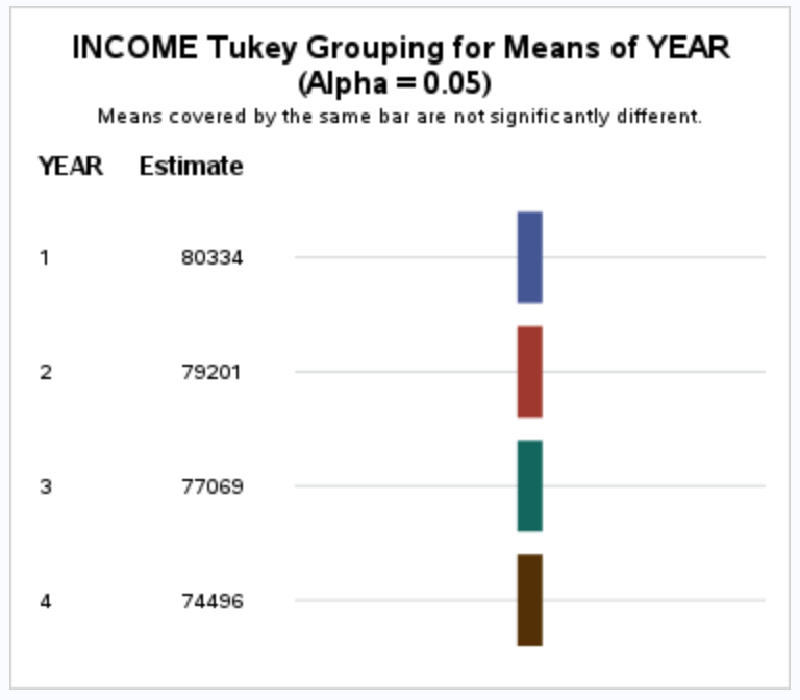
\includegraphics[width=\textwidth]{Income by year.pdf}
  \caption{This is my first figure.}\label{fig:cars}
\end{figure}

\section{Discussion}\label{sec:disc}

What are the main contributions again?

What are the limitations of this study?

What are worth pursuing further in the future?


\appendix

\bibliography{../manuscript/ref}
\bibliographystyle{chicago}

\end{document}

{housing by income.pdf}
{housing by year.pdf}
{Income by town.pdf}
{Inome by year.pdf}
{Rehosp by income/year.pdf}
{Stamps by income/year.pdf}